\documentclass[12pt]{article}
%\usepackage[showframe]{geometry}% http://ctan.org/pkg/geometry
\usepackage{lipsum}% http://ctan.org/pkg/lipsum
\usepackage{multicol}% http://ctan.org/pkg/multicols
\usepackage{graphicx}% http://ctan.org/pkg/graphicx
\usepackage{fancyhdr}
\usepackage{titling}
\usepackage{subcaption}
\usepackage{indentfirst}
\usepackage{booktabs}
\usepackage{multirow} 
\usepackage{setspace} \doublespacing
\usepackage{mathptmx}
\usepackage[backend=biber, style=apa,]{biblatex}
\usepackage{hyperref}

\pagestyle{fancy}
\doublespacing

\addbibresource{/mnt/c/Users/woute/Zotero/My Library.bib}

\hyphenpenalty=1000
\tolerance=2000

\fancyhead{}
\fancyfoot{}
\fancyfoot[R]{\thepage}
\renewcommand{\headrulewidth}{0pt}

\setlength{\droptitle}{-10em}   % This is your set screw

\begin{document}

\begin{titlepage}
\centering

% Adjust font size and family as needed
{\LARGE\bfseries Local Circuit Structure of Mouse Visual Cortex for Generating Illusory Contour Responses\par}

\vspace{5pt} % Adjust space between title and figure as needed

% Include the figure

\includegraphics[width=0.5\textwidth]{figures/donders_logo.png}

\includegraphics[width=0.5\textwidth]{figures/uva_logo.png}


\vspace{20pt} % Adjust space between figure and author/date as needed

% Author and Date
{\Large Wouter Kroot\par}
\vspace{5pt} % Adjust as needed
{\Large April 2024\par}
\vspace{5pt}
{\Large Supervisor: Prof. dr. P.H.E. Tiesinga}

\end{titlepage}

% Rest of the document starts here
\newpage

% Abstract
\begin{abstract}
  \lipsum[1]
\end{abstract}

\newpage

\section{Introduction}
\subsection{Illusory contour and visual segmentation.}
The representation and identification of visual contours is an essential step in order to perceive coherent objects with respect to each other and the background.
In some cases, visual contours are clearly defined, e.g., by a luminance contrast that indicates a discontinuity. In other cases, other figures occlude contours, 
and objects must be partly inferred from locally available visual cues. Interestingly, particular stimulus configurations can give rise to the perception of contours 
that are not physically present. For example, the 'abutting grating' and 'Kanizsa' illusions (Figures 1 and 2). These illusory contours are a product of visual interpolation that signals the presence of an occluding figure. Although the perception of these geometrical shapes is seemingly simple, both illusions require a process that analyses the discontinuities of the inducing lines and assesses their relation towards each other. Typically, an illusory line is only formed when the connected edges form a closed contour and are interpreted as part of the foreground. Since these illusory contours are not physically present and are a direct product of our neural circuitry, illusory contours can  effectively be used to investigate the underlying neurophysiological interactions necessary to make perceptual inferences. Although there are many different stimulus configurations  that can elicit illusory contours, neurophysiological research has mainly focused on the abutting grating illusion and the Kanizsa triangle illusion. The results of both illusions will be discussed since their underlying neural mechanisms are likely similar. In order to make the results from current simulations as clear as possible, the choice was made only to use the abutting grating illusion and not Kanizsa. Furthermore, the goal of the current model is to further explain the cortical representation of illusory contour by explicitly modelling receptive fields along the visual pathway, trying to account for the most important constraints posed by mammalian neurophysiology.

\bigbreak

The initial neuronal evidence of illusory contours was identified in V2 neurons of alert rhesus macaques \autocite{vonderheydtMechanismsContourPerception1989}.
%\autocite{vonderheydtMechanismsContourPerception1989}. %(von der Heydt \& Peterhans, 1989). 
To elicit the abutting gratings illusion, offset lines were presented in an abutting pattern with overlapping ends (see Figure 1). This research highlighted 
a distinct difference between the primary visual  cortex (V1) and the secondary visual cortex (V2). It was discovered that V1 plays a minimal role in the representation of illusory contours, with nearly all orientation-selective neurons (59 out of 60) showing no activity related to the orientation of the illusory contours. In contrast, a significant number of neurons in V2 (45 out of 103, or approximately 44\%) did respond to the orientation of illusory contours, signifying that V2 represents the initial cortical area where illusory contours are detected. Furthermore, it was observed that many V2 neurons displayed similar orientation tuning for both real and illusory contours. However, there were also neurons that responded to both real and illusory contours at  orientations diverging by up to 90 degrees. These observations demonstrate the visual system's capacity to represent information beyond the mere activation by direct sensory input. Illusory contours entail advanced processing, wherein the brain infers the existence of contours from the local visual cues provided and sends feedback to the lower visual areas. 
This inferential process is essential for forming a coherent perception of the visual environment, allowing the visual system to interpolate missing segments and interpret ambiguous or incomplete visual scenes.
  
\begin{figure}
    \centering
    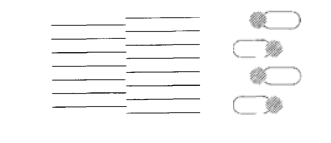
\includegraphics[width=0.95\textwidth]{figures/simple_abutting.png}
    \caption{Abutting grating illusion (Soreano et al., 1996), the offset between the lines gives the impression of a vertical contour overlapping the horizontal inducers. 
    The proposed neural mechanism is the integration of endstopped cells, which can be characterised by an elongated excitatory receptive field and inhibitory endzones.}
    \label{fig:figure_1}
\end{figure}

\bigbreak
\subsection{Neural mechanism macaque V4 and mice V1-LM.}
Macaque V2 cells' showed that their tuning to illusory contours is not necessarily the same as the orientation tuning to real contours, which suggests a potential mechanism where feedback signals may determine V2 cells' orientation selectivity towards illusory contours. If the orientation tuning to illusory contours were indeed a result of feedback, a direct implication would be that higher visual areas might be unable to distinguish between real and illusory contours. This hypothesis has been examined, with area V4 in the macaque identified as a crucial integration point where both real and illusory contours are represented equivalently \autocite{panEquivalentRepresentationReal2012}. Through the use of optical imaging and single-cell recordings to compare neural activity elicited by real and illusory contours across areas V1, V2, and V4, it was found that activities in V1 and V2 predominantly relate to the encoding of local spatial features of the inducers, rather than the global orientation of the illusory contour. Meanwhile, V4 processed both real and illusory contours similarly, indicating that hierarchical interactions might govern the global orientation processing of illusory contours. This suggests that feedback mechanisms could account for the selective stimulation and orientation tuning of V2 cells in response to illusory contours.
\bigbreak

Additional support for the vital role of feedback in the representation of illusory contours is provided by studies illustrating the interactions between V1 and the lateromedial visual area (LM) in mice during the perception of illusory contours \autocite{pakTopDownFeedbackControls2020}. These studies trained mice to differentiate between stimuli with and without illusory contours, linking their behaviour to neural activity (Figure 2). Given the extensive genetic tools available for mice that allow for the precise recording and stimulation of specific cells, they are exceptionally well-suited for investigating the hierarchical processing that underpins perceptual inferences. The findings revealed that, akin to macaques, mice also exhibited a delay (30 ms) in the representation of illusory contours compared to those defined by contrast, suggesting that the processing of illusory contours involves a more complex integration of visual information than that of contours directly derivable from sensory input. Moreover, the representation of illusory contours in V1 was eliminated upon the silencing of LM through optogenetics, indicating a possible similarity in the processing relationship between V1 and LM in mice and that between V2 and V4 in macaques, which aligns with theories of recurrent processing \autocite{wyatteEarlyRecurrentFeedback2014}. Additionally, recent research \cite{shinRecurrentPatternCompletion2023} found that a specific subset of V1 cells in mice could complete the perception of an illusory contour when sufficiently stimulated. Employing decoding techniques and 2-photon stimulation, it was demonstrated that activating a particular set of V1 cells could suffice to generate the perception of illusory contours across the V1 network, even without any visual stimulus. These findings underscore the significance of recurrent activity in the representation of illusory contours and highlight the necessity for further investigation into how these cells are precisely targeted based on the configuration of inducing stimuli.

\begin{figure}
    \centering
    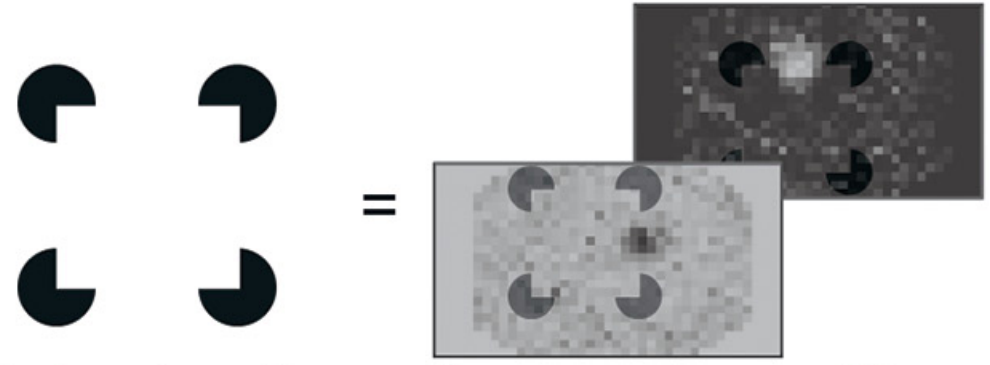
\includegraphics[width=0.95\textwidth]{figures/Kanizsa_Mice.png}
    \caption{Kanizsa illusion (Pak et al., 2020), four spatially synchronous pac-men that induce the impression of a white square overlapping four circles, inducing the percept of a not physically present contour. When presented to mice, orientation-selective cells show activity along the length of the illusory line.}
    \label{fig:simple_abutting}
\end{figure}

\bigbreak
\subsection{Endstopped cells fundamental to illusory contour representation.}
The abutting grating and Kanizsa illusions are both characterized by congruent illusory inducing points, identifiable by the presence of aligned line endings. Kanizsa inducers are considered more complex than abutting line inducers because each inducer point forms part of a corner, essentially two line ends meeting at an angle. In contrast, the abutting grating illusion is simpler, with its inducer points as single-line ends and, therefore, could be represented by a single endstopped cell \hyperref[fig:figure_1]{(figure 1)}.
Nonetheless, cells sensitive to length might be fundamental to encoding both illusions, known as endstopped cells. Initially classified by Hubel and Wiesel in the cat's primary visual cortex (V1) in 1969, these cells are orientation-tuned and exhibit inhibition when a line segment exceeds their excitatory receptive field, leading to their initial characterization as hypercomplex cells for their complex cell properties, such as stimulus polarity invariance, combined with inhibitory end zones \autocite{hubelRECEPTIVEFIELDSFUNCTIONAL1965}. Subsequent research revealed that a significant portion of V1 neurons exhibit endstopping to varying degrees  \autocite{deangelisLengthWidthTuning1994,jonesSurroundSuppressionPrimate2001,sceniakVisualSpatialCharacterization2001} across different species, including primates, cats, and mice. Computational models have shown that endstopping can sufficiently delineate figures from the background and reconstruct illusory contours \autocite{vonderheydtMechanismsContourPerception1989}, suggesting that endstopped cell integration might serve as a universal neural mechanism for segmenting the visual field and to generating illusory contours.

\textbf{Image segmentation between mice and macaque have different straties, luongo 2023, both are suitable for endstopping.}

\begin{figure}
  \centering
  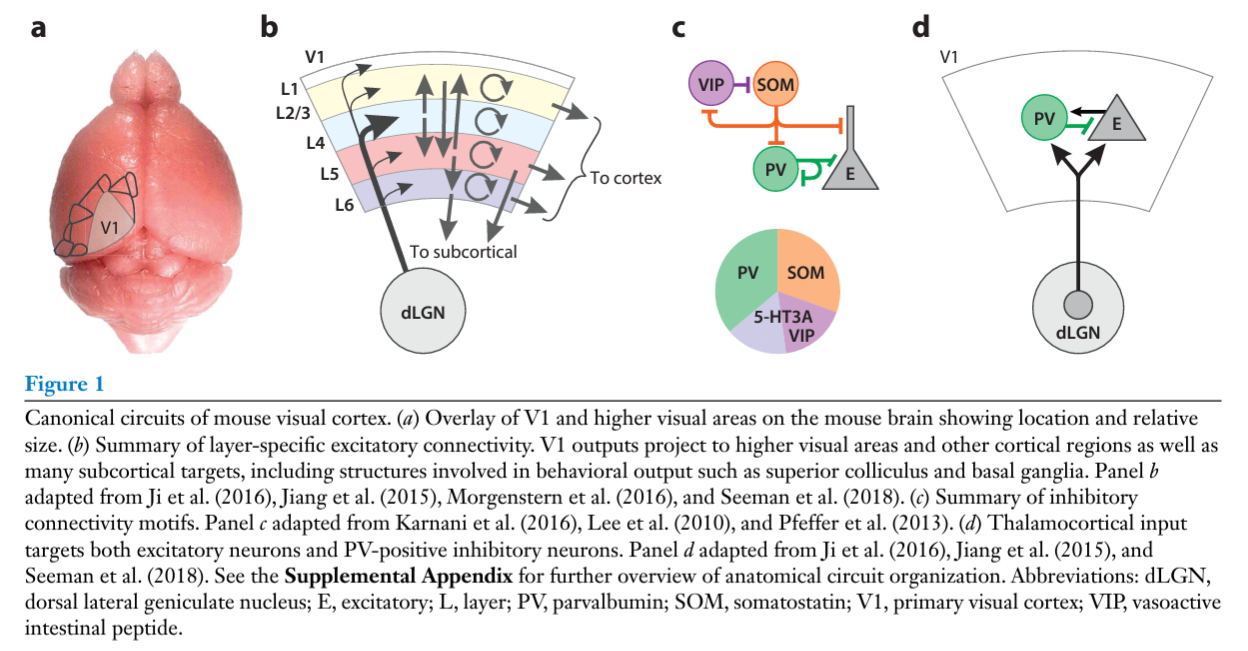
\includegraphics[width=1.0 \textwidth]{figures/Canonical_laminar_projection.png}
  \caption{laminar projections similar from apes and mice?, from Niell, Scanziaini, 2021 Annual Review}
  \label{fig:figure 3}
\end{figure}

\bigbreak
\subsection{Current study.}
Despite these insights, neurophysiological studies have largely overlooked how endstopping is integrated into higher visual areas for illusory contour perception. Previous computational simulations, while informative, have relied on feed-forward convolutions without accounting for biological constraints, such as direct inhibition to simulate negative end zones (Sillito \& Versiani, 1977), and have not incorporated feedback mechanisms now recognized as crucial for the representation of illusory contours in lower visual areas.

Addressing this gap, our current research endeavours to simulate endstopping using Leaky Integrate and Fire (LIF) neurons and to integrate endstopped microcircuits through population rate models to accurately represent the abutting grating illusion. Our findings shed light on the minimal microcircuit necessary to exhibit end-stop characteristics, further illuminating how the representation of illusory contours through recurrent activity is modulated by the orientation selectivity of endstopped cells in higher visual areas. By incorporating endstopped cells into a hierarchical model, we aim to elucidate the neural mechanisms underlying illusory contour perception and to provide a comprehensive understanding of how the visual system processes illusory contours.

This study investigates whether endstopping in V1 can occur solely through feedforward signals without direct inhibition or if a feedback mechanism is essential for activating inhibitory end zones. By simulating the representation of the abutting grating illusion via endstopped cell-driven recurrent activity, we explore the physiological constraints on integrating orientation-tuned endstopped cells in higher visual areas. Our goal is to elucidate how endstopped cells contribute to the perception of illusory contours and their integration within the visual cortex hierarchy. We hypothesize that endstopped cells are crucial for the representation of illusory contours and that their orientation tuning is modulated by feedback signals from higher visual areas. Our results will provide insights into the neural mechanisms underlying illusory contour perception and the hierarchical processing of visual information in the mammalian visual system.

\newpage
\section{Methods}
% Introduction that states that we used two models with a rationalisation of why
\noindent \textbf{Spiking neuron and population Model design.} \newline
To investigate the local circuit necessary for endstopping and how endstopping features can be used to generate illusory contours within the visual cortex of the mouse, the current study used two distinct computational frameworks. In the initial phase of the investigation, we utilised leaky integrate-and-fire (LIF) models to simulate the spatial and temporal integration of synaptic input, on the single-cell level. This approach provided a foundational understanding of the mechanisms underpinning orientation selectivity, complex cell features such as polarity invariance, and endstopping. However, the current connectivity between LIF cells was set by hand, and the complexity and computational demands associated with the tuning of each neuron constrained the current study to shift towards population models for the subsequent phase of generating illusory contours. Nevertheless, the LIF network allowed an estimate of the necessary amount of cells needed to create a stable neural mechanism for endstopping, and the population models could abstract this behaviour into a computationally tractable form, enabling the simulation of illusory contour generation efficiently. 

\bigbreak
\subsection{Simulating the Local Circuit for Endstopping.}

To stimulate endstopping behaviour the Brain Modeling Toolkit was utilised to define and connect nodes. To construct an architecture of spiking point neurons it is necessary to initilialise an instance of the NetworkBuilder class provided by the BMTK. The current example will create a network for the dLGN and a network for V1.

To present the visual stimuli and connect nodes from the LGN to V1, the Brain Modelling Toolkit was used. This simulation pipeline processed visual information through a series of steps with increasing complexity, starting with presenting the visual stimulus. Visual stimuli were dynamically presented through a three-dimensional array format (t, y, x). Each entry along the first dimension time (t) is a frame with input organised along the vertical (y) and horizontal (x) dimensions. 

By following these steps, you can effectively use the Brain Modeling Toolkit to create complex neural networks. The toolkit's flexibility allows for precise control over the spatial arrangement and connectivity of neurons, facilitating the modeling of intricate neural circuits and their dynamic behaviors. This guide demonstrates the process of defining, connecting, visualizing, and saving neural networks using BMTK, providing a robust framework for neural network modeling and simulation.

An important aspect of BMTK is its support for different simulation environments. In this context, we used two distinct types of simulations: filternet and pointnet. Filternet is employed to simulate the LGN, focusing on the filtering properties of LGN neurons and their responses to visual stimuli. This separate simulation environment is particularly suited for capturing the dynamics of large-scale LGN networks and their pre-processing role in the visual pathway. The importance of using filternet lies in its ability to model the initial stages of visual processing, where the LGN acts as a relay station, refining and filtering visual information before it reaches the cortex. This simulation environment allows for detailed analysis of how LGN neurons process various visual inputs and contribute to the overall visual perception.

On the other hand, pointnet is used to simulate the V1 network with the NEST simulator. NEST is well-suited for modeling spiking neural networks and supports the integration of point-neuron models, making it ideal for simulating the detailed spiking activity and synaptic interactions within the V1 network. By using pointnet, we can leverage NEST's capabilities to simulate the complex dynamics of V1 neurons, including their interactions and the resultant network behavior. The importance of using pointnet lies in its ability to model the cortical processing of visual information, where the integration of inputs from the LGN and the intrinsic cortical circuitry results in the emergence of complex visual features such as orientation selectivity and phase invariance.

By separating the simulations into filternet for the LGN and pointnet for the V1 cortex, we can more accurately model the distinct roles these regions play in visual processing. Filternet allows for a focused examination of the LGN's filtering mechanisms, while pointnet provides a detailed simulation of cortical processing dynamics. This approach ensures that each component of the visual pathway is modeled with the appropriate level of detail, leading to more accurate and comprehensive simulations of visual processing.

% Overview figure
\begin{figure}[htbp!]
  \centering
  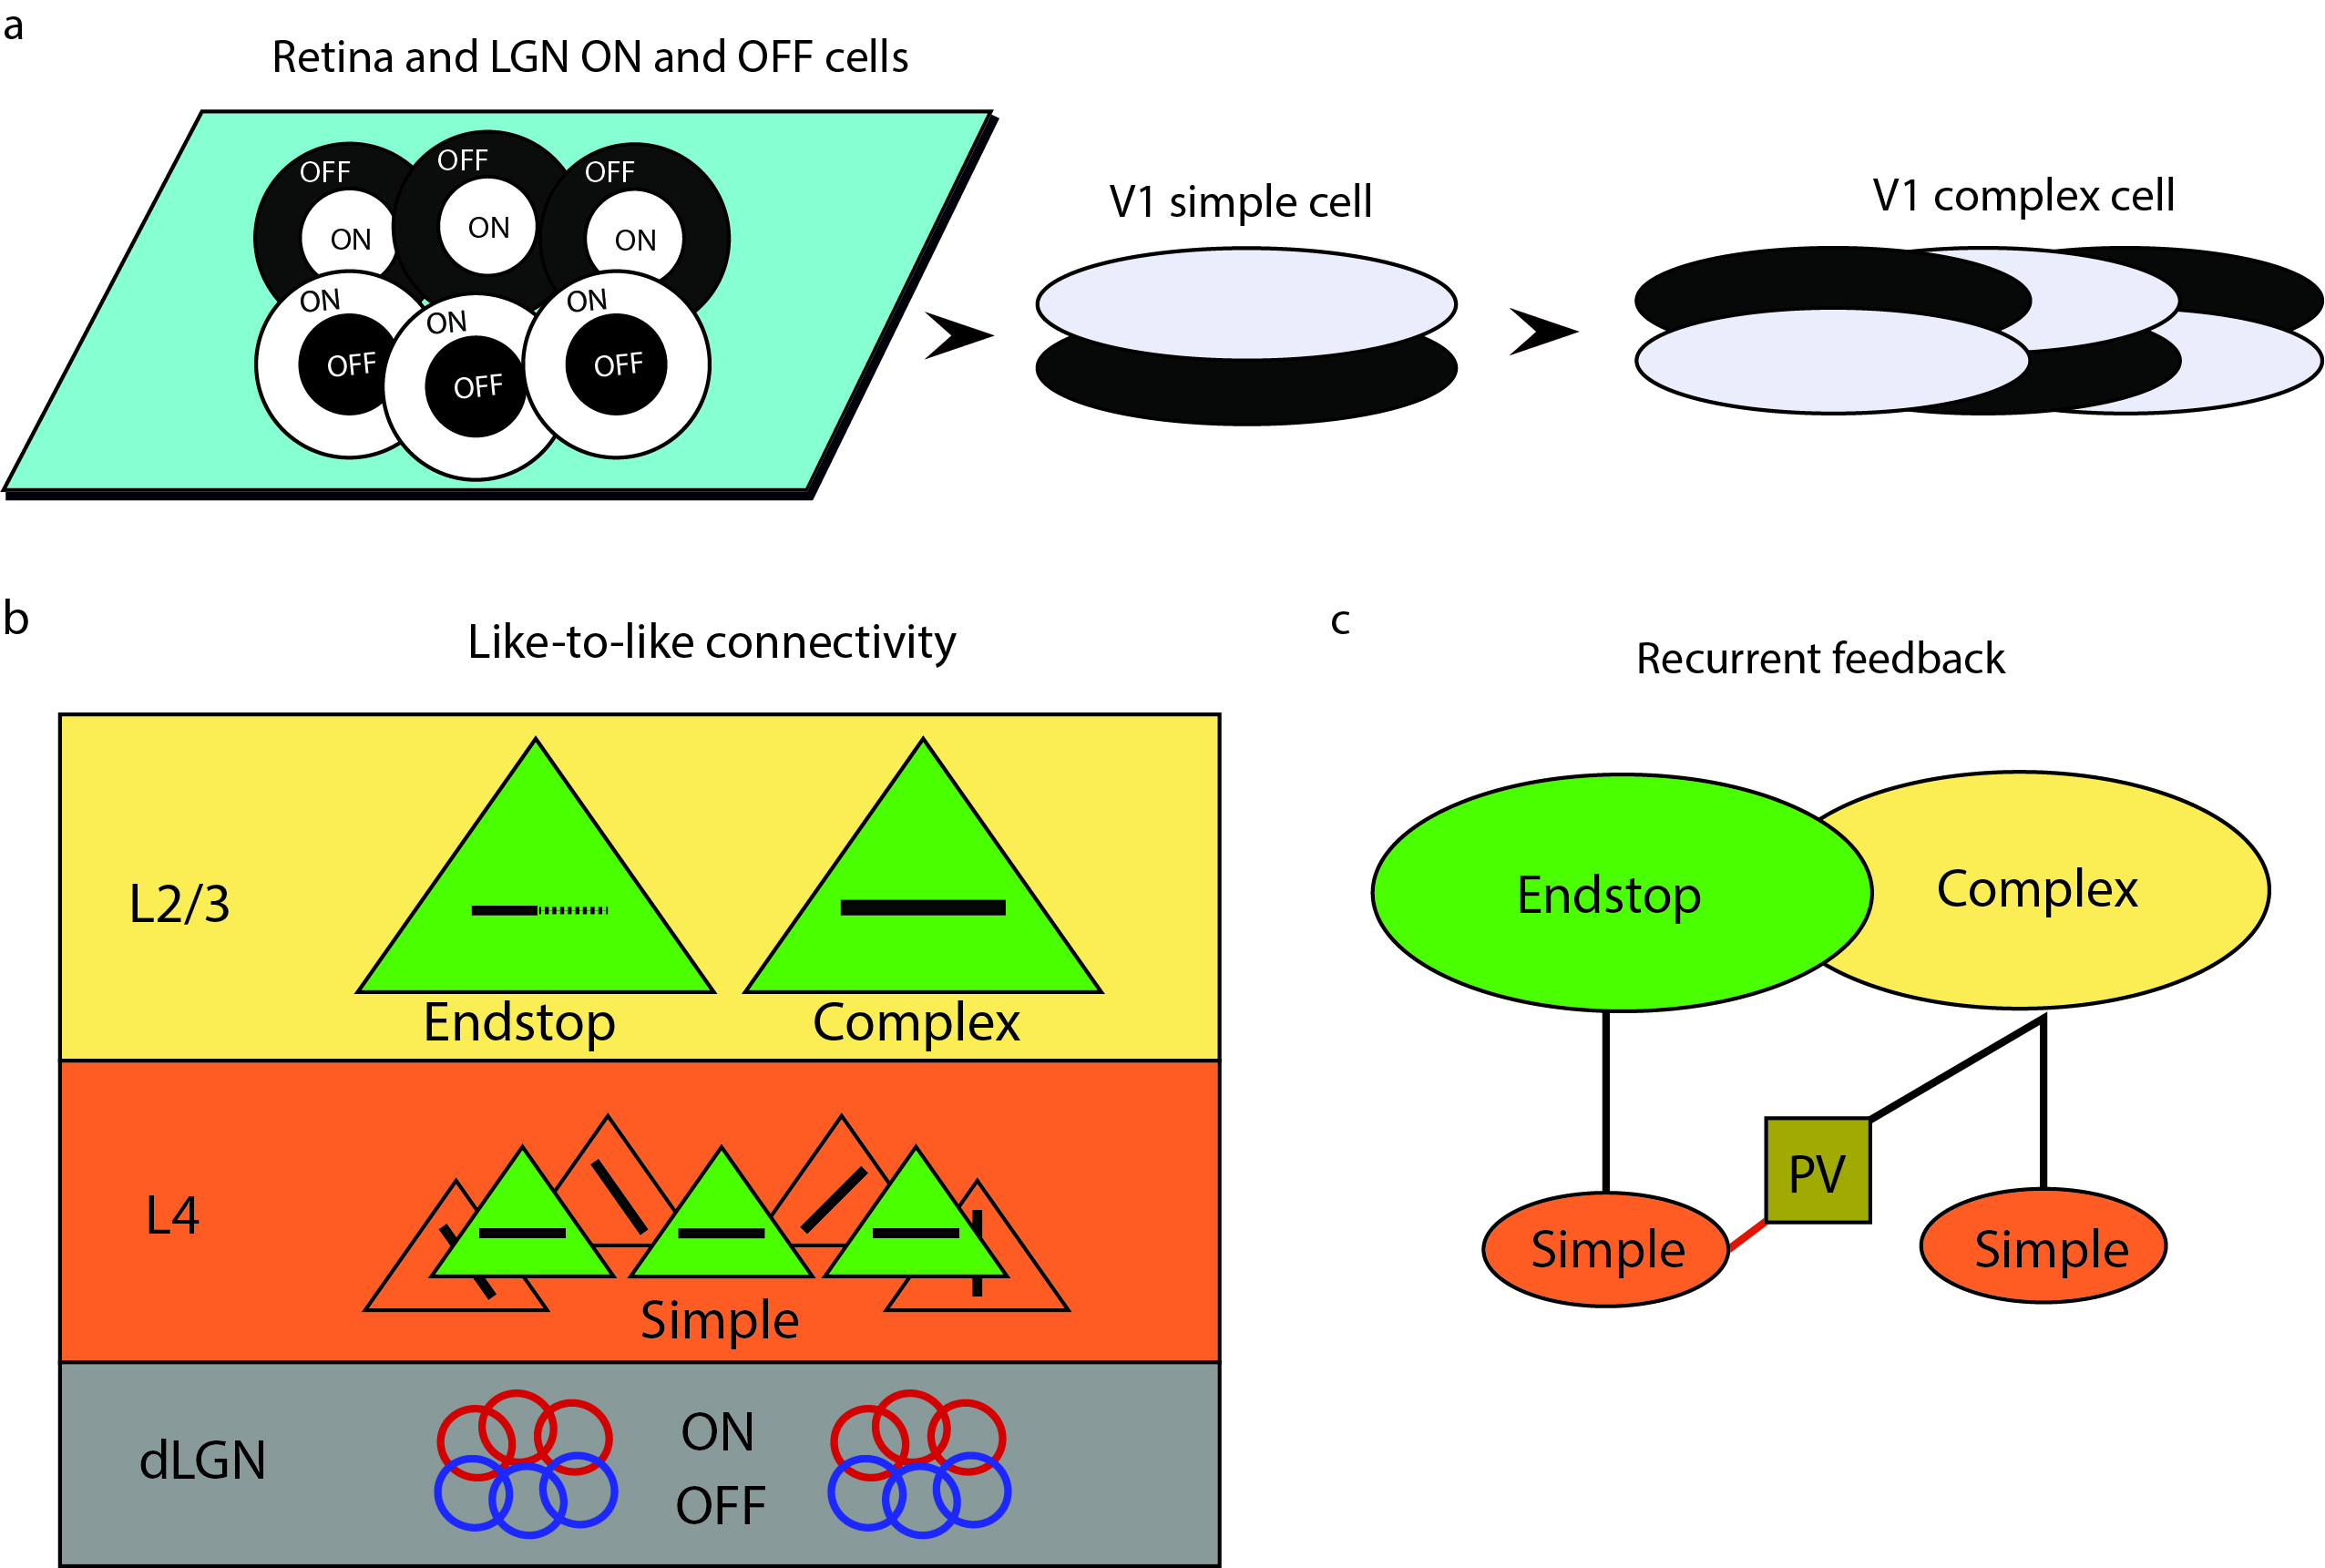
\includegraphics[width=1.0 \textwidth]{figures/overview.jpg}
  \caption{Best to change a to Retina dLGN ON and OFF surround cells}
  \label{fig:LIF connectivity}
\end{figure}

\bigbreak
\textbf{Table with LGN, simple and complex parameters.}

\begin{table}[h!]
\centering
\caption{Parameters and Weights for LGN and V1 Cells}
\begin{tabular}{lll}
\toprule
\textbf{Cell Type} & \textbf{Parameter} & \textbf{Description} \\
\midrule
\multirow{4}{*}{LGN} 
    & Optimized weight      & 10, -1 \\
    & Parameter bounds   & P \\
    & Delays   & 0, 5 \\
    & K-peaks   & 54, 127 \\
\midrule
\multirow{6}{*}{V1} 
    & External current         & 0.0 nA \\
    & Membrane time constant        & 44.9 ms \\
    & Membrane capacitance          & 239.0 pF \\
    & Refractory period       & 3.0 ms \\
    & Resting potential          & -78.0 mV \\
    & Threshold potential         & -43.0 mV \\
    & Reset potential      & -55.0 mV \\
\bottomrule
\end{tabular}
\end{table}

\subsection{Orientation Selectivity in V1}
Our study aimed to achieve orientation selectivity in V1 simple cells by strategically connecting LGN cells to them using elliptical receptive fields. Specifically, we designed each simple cell in V1 to have a receptive field composed of two distinct elliptical regions: one for ON and one for OFF responses. These ellipses were positioned relative to each other and oriented along a specific angle, allowing the V1 cells to sample input selectively from ON and OFF LGN cells.

To implement this, we first defined the receptive field for each V1 simple cell by setting the parameters of the ellipses. Each ellipse had a specific orientation, which was determined by the angle of its major axis, reflecting the preferred orientation of the V1 cell. The separation between the centres of the ON and OFF ellipses was carefully specified to ensure that these regions were spatially distinct but aligned according to the desired orientation. This separation allowed the ON and OFF regions to be positioned so they could selectively sample from the respective ON and OFF LGN cells.

Connections from the LGN cells to the V1 simple cells were established using a selective connection rule implemented through a connection function. This function determined whether an LGN cell's position fell within the bounds of the ON or OFF ellipse of a given V1 cell. For each LGN cell, the function checked if the cell's position was within the elliptical boundary using a mathematical condition that defines whether a point lies inside an ellipse. This condition was based on the ellipse's centre, axes, and orientation, allowing precise determination of the inclusion of LGN cells within the receptive fields of the V1 cells.

Once an LGN cell was identified as being within the receptive field of a V1 cell, synaptic connections were established with specific weights and delays. These synaptic parameters were carefully tuned to reflect the physiological properties of synaptic transmission observed in biological systems. The synaptic weights determined the strength of the input from the LGN cell to the V1 cell, while the delays accounted for the time taken for the signal to travel between the two cells.

The network construction involved creating a V1 network with simple cells characterized by their orientation, positions, and receptive field parameters, such as the separation between ellipses, the radius, and the aspect ratio of each ellipse. The positions of the V1 cells were generated within a specified spatial grid to simulate the realistic arrangement of neurons in the visual cortex. Similarly, the LGN cells were distributed across a spatial grid with their positions randomly generated within defined bounds, reflecting the natural variability in the spatial distribution of these cells.

The selective connection rule played a crucial role in achieving orientation selectivity. The rule iterated over all possible LGN sources for each V1 target, checking for inclusion within the ellipses and establishing connections accordingly. This process ensured that each V1 simple cell received input from a specific subset of LGN cells aligned with its receptive field configuration. By connecting each V1 cell to a well-defined set of ON and OFF LGN cells, the V1 cells could respond preferentially to specific orientations of visual stimuli.

Through this method, elliptical receptive fields with distinct ON and OFF regions enabled the V1 simple cells to become orientation-selective. The careful design of the spatial arrangement of the ellipses, combined with the selective connection rules, ensured that the V1 cells exhibited orientation selectivity similar to that observed in biological visual systems. This approach provided a robust model for studying the mechanisms of orientation selectivity and the role of specific LGN inputs in shaping the response properties of V1 neurons.

\begin{figure}[htbp!]
    \centering
    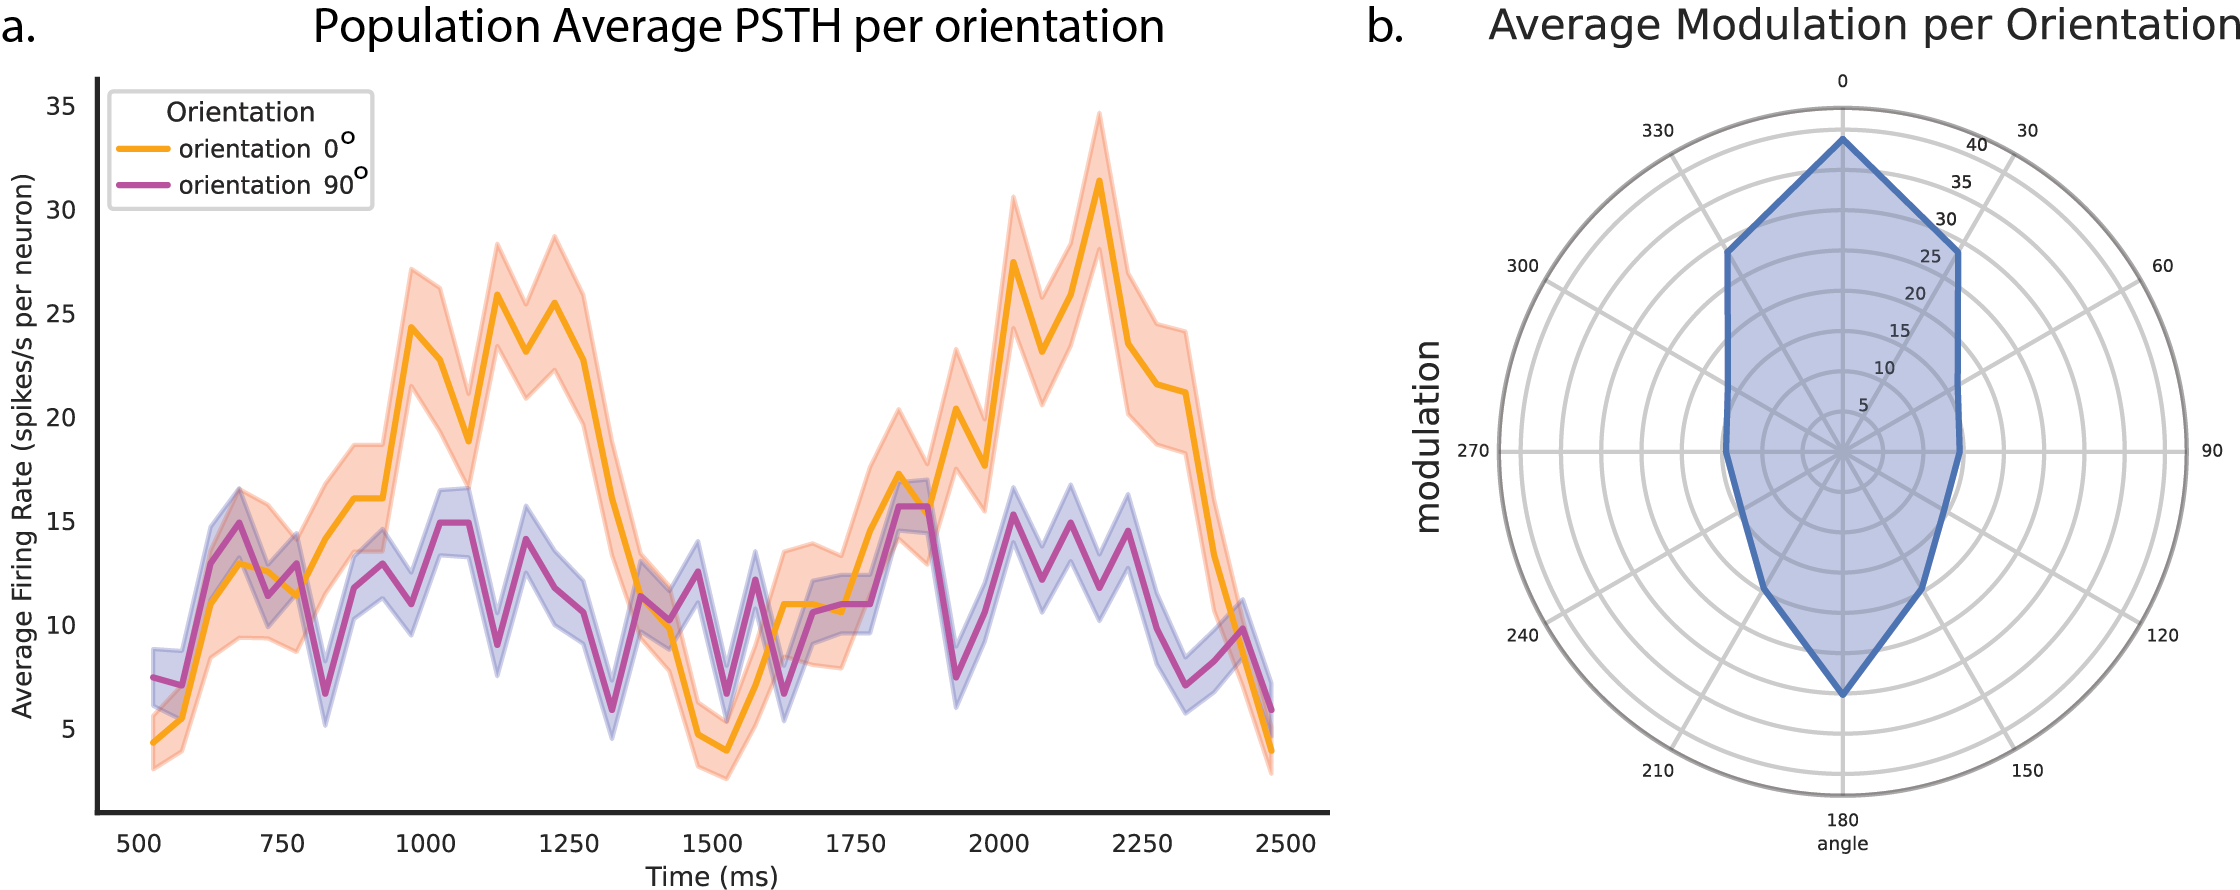
\includegraphics[width=1 \textwidth]{figures/figure_simple_orientation_tuning.png}
    \caption{Orientation tuning example of population ON/OFF cells at 0 and 90 degrees. The idea is to make a raster plot of the 90 a path and average modulation plot, then the same for the 0 degrees. So we have raster, under that psth  for both the 0 and the 90 degrees, and next to that a large orientation polar plot for all orientations}
    \label{fig:simple cell orientation tuning}
\end{figure}

\subsection{Polarity Invariance of Complex Cells.}
Subsequently, complex cells are created by strategically connecting these simple cells. The process began by connecting LGN cells to V1 simple cells using elliptical receptive fields and then by combining simple cells to form complex cells; we ensured phase invariance and enhanced orientation selectivity.

Connections from LGN cells to V1 simple cells were established using a selective connection rule implemented through a connection function. This function determined whether an LGN cell's position fell within the bounds of the ON or OFF ellipse of a given V1 cell. For each LGN cell, the function checked if the cell's position was within the elliptical boundary using a mathematical condition defining point inclusion inside an ellipse based on the ellipse's centre, axes, and orientation. Once identified within the receptive field of a V1 cell, synaptic connections were established with specific weights and delays. These synaptic parameters were tuned to reflect the physiological properties of synaptic transmission observed in biological systems, with synaptic weights determining the strength of the input and delays accounting for the signal travel time between the cells.

 The next step involved creating complex cells from retinotopically aligned ON/OFF and OFF/ON simple cells. This was achieved by converging multiple simple cells with the same preferred orientation but different spatial phases onto a single complex cell. The key to achieving phase invariance in complex cells lies in the convergence of inputs from simple cells that are sensitive to the same orientation but have different phase preferences.

The selective connection rule played a crucial role in this process. The rule iterated over all possible simple cell sources for each target complex cell, checking for alignment in orientation and differences in phase. Synaptic connections were established between the simple cells and the complex cell, ensuring that the complex cell received inputs from a diverse set of simple cells. This convergence allowed the complex cell to respond to a range of spatial phases of a given orientation, thereby achieving phase invariance.

In the code implementation, complex cells were created by defining their receptive fields and connecting them to simple cells using a similar selective connection rule. The positions of complex cells were generated within a specified spatial grid, and their receptive fields were aligned with the preferred orientations of the contributing simple cells. The connection rule ensured that each complex cell received input from multiple simple cells with the same orientation preference but different phase preferences. This was accomplished by iterating over all potential simple cell sources for each target complex cell, establishing connections based on the orientation and phase alignment.

Through this method, elliptical receptive fields with distinct ON and OFF regions enabled V1 simple cells to become orientation-selective. By combining these simple cells to form complex cells, we achieved phase invariance, allowing complex cells to respond robustly to a given orientation regardless of the spatial phase of the input. The careful design of the spatial arrangement of the ellipses, the selective connection rules, and the convergence of simple cells onto complex cells ensured that the V1 network exhibited properties similar to those observed in biological visual systems. This approach provided a robust model for studying the mechanisms of orientation selectivity, phase invariance, and the role of specific LGN and simple cell inputs in shaping the response properties of V1 neurons.

\begin{figure}[htbp!]
    \centering
    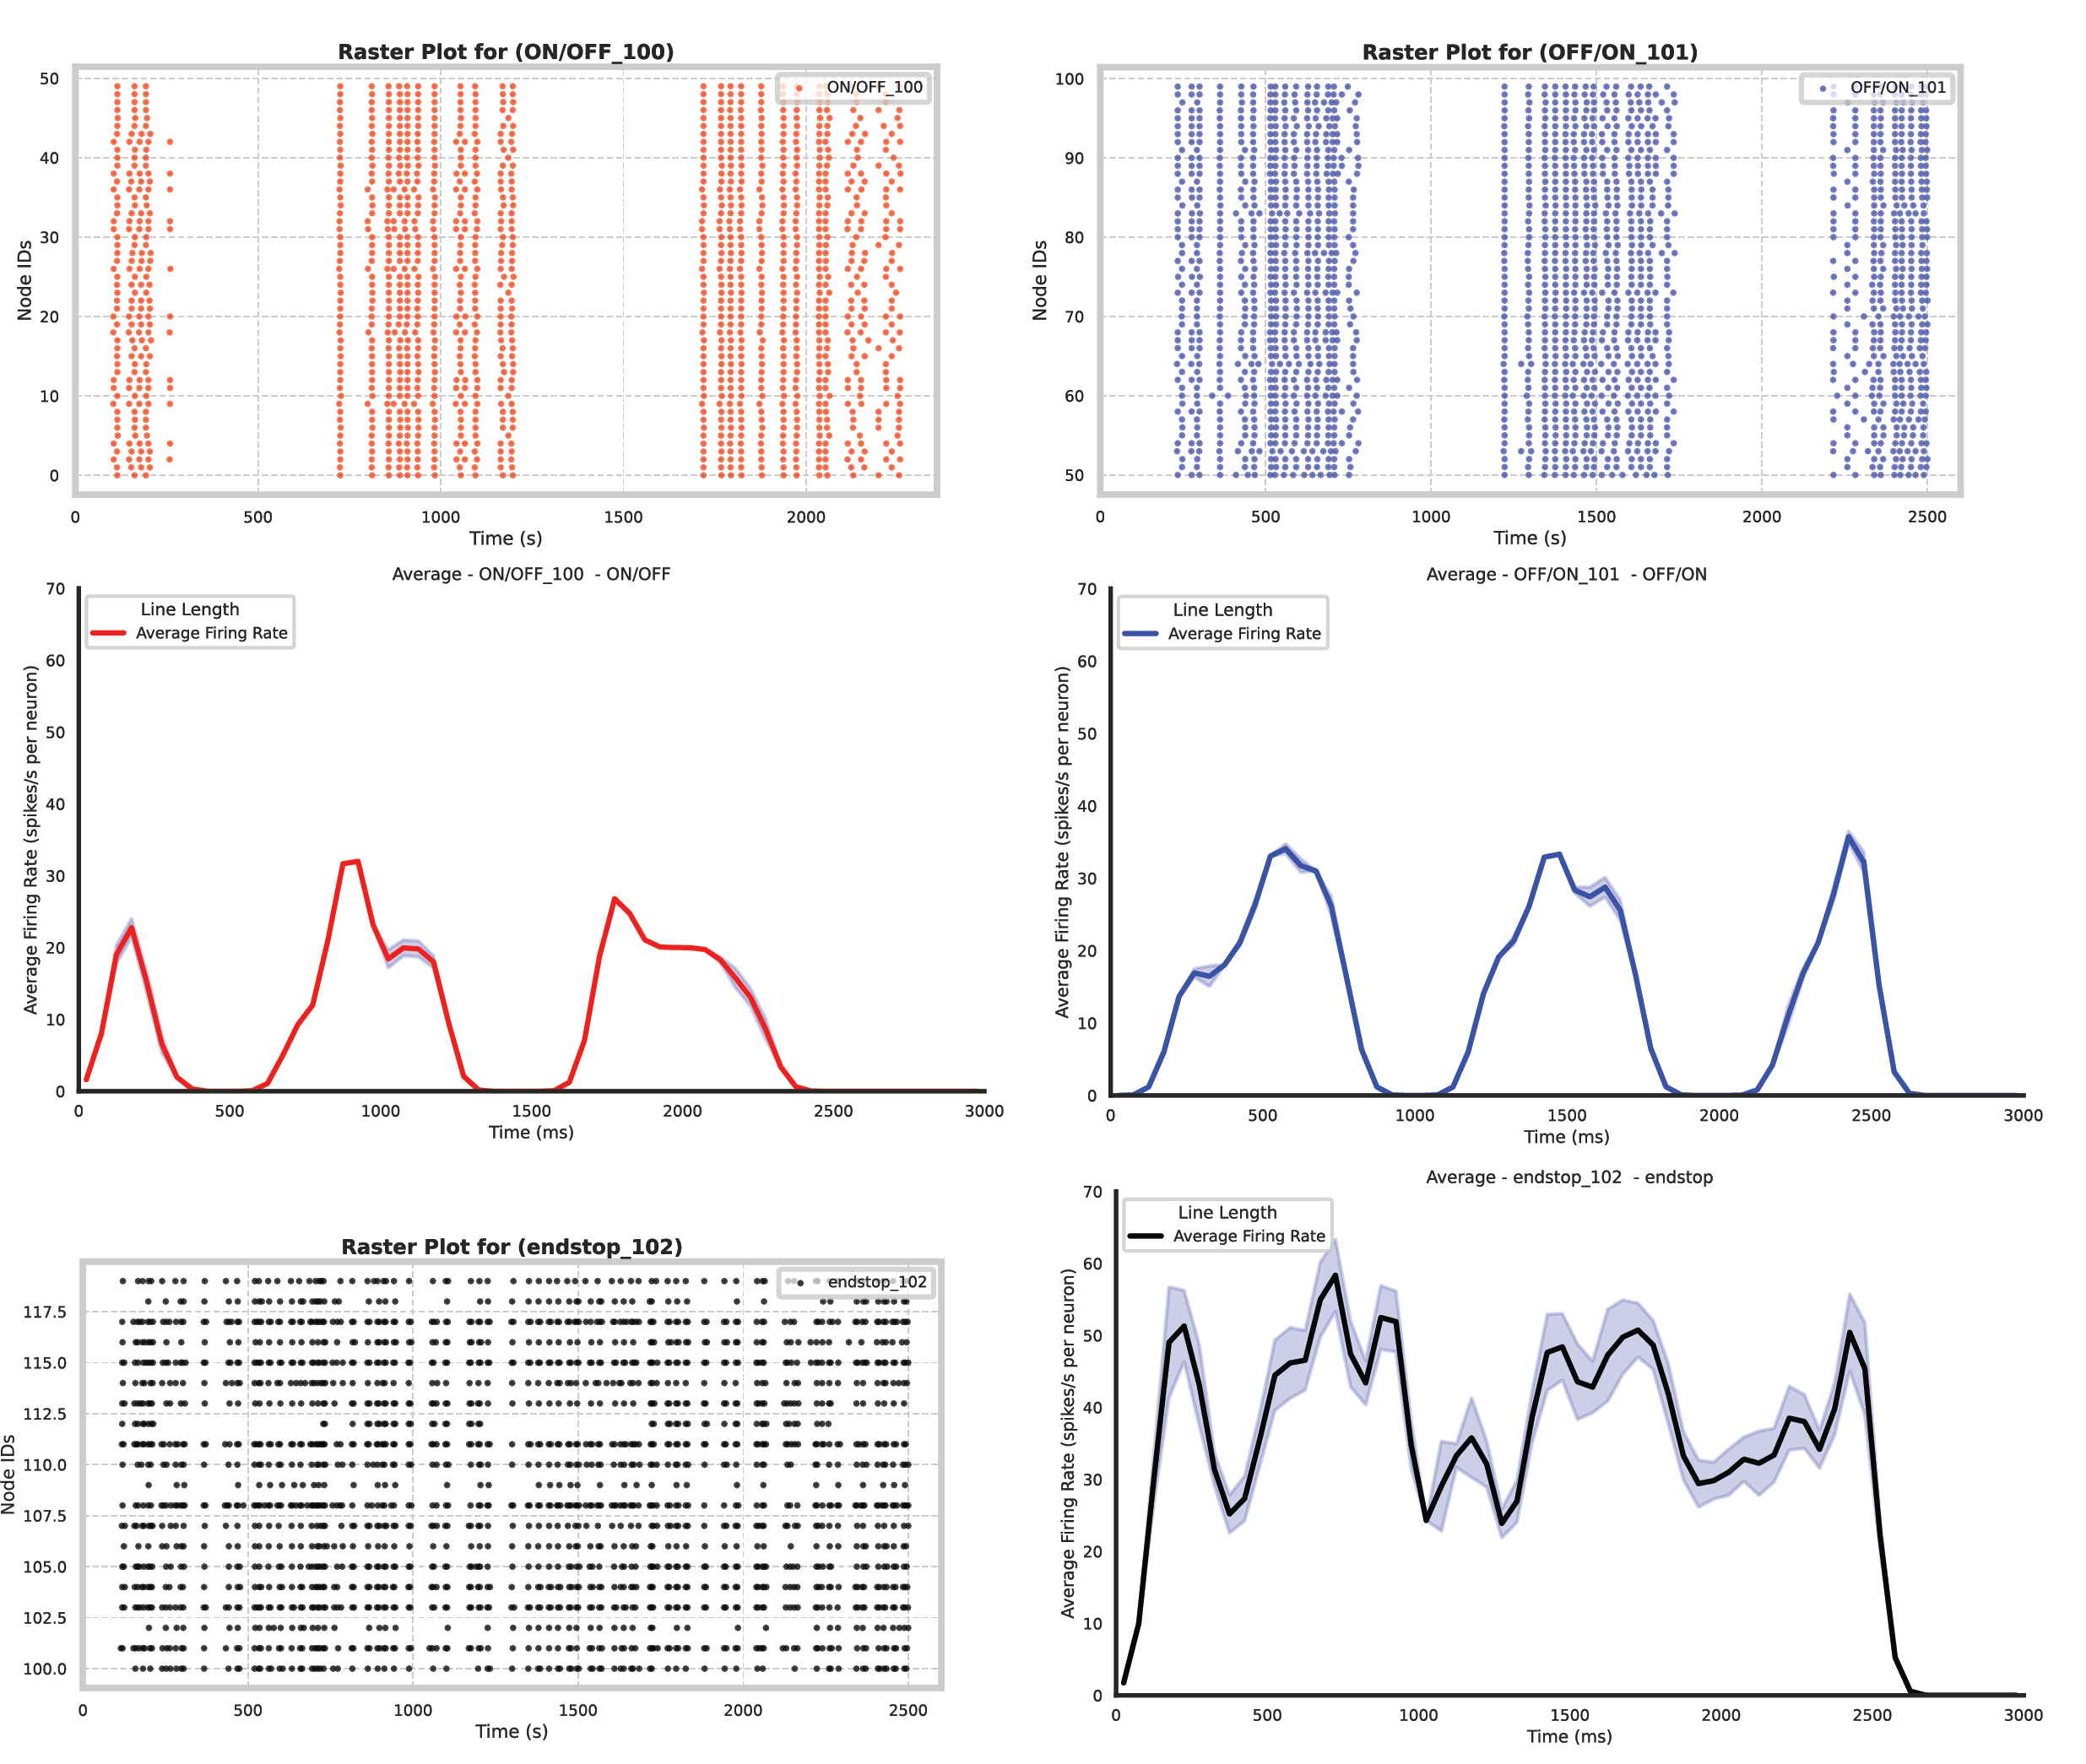
\includegraphics[width=1 \textwidth]{figures/Complex_invariancy.png}
    \caption{Polarity invariance of complex cells, 0 and 90; while maintaining the right orientation selectiveness}
    \label{fig:polarity invariance}
\end{figure}

\subsection{Recurrent feedback underlying endstopping.}
In addition to creating orientation-selective and phase-invariant complex cells, I employed recurrent feedback to inhibitory cells to model the phenomenon of endstopping, a critical feature in the visual processing system. The process began with the projection of simple cells into complex cells. Specifically, simple cells with orientation-selective receptive fields were connected to complex cells that integrated inputs across different spatial phases, thus achieving phase invariance.

The next step involved the lateral displacement of these complex cells. These laterally displaced complex cells then projected to inhibitory interneurons. This displacement was crucial as it introduced a spatial offset between the excitation source and the location where inhibition would be applied, mimicking the spatial dynamics observed in cortical circuits. The inhibitory interneurons targeted by these projections played a key role in modulating the activity of the simple cells.

Once activated by the complex cells, the inhibitory cells provide feedback to the simple cells positioned directly beneath the original complex cells. This feedback loop was designed to suppress the activity of the simple cells when a stimulus extended beyond their receptive field. In more detail, as a line or bar stimulus moved across the receptive field of a simple cell and extended beyond it, the laterally displaced complex cell would activate the inhibitory interneurons. These interneurons, in turn, would inhibit the simple cells, thereby reducing their firing rate. This rapid inhibition is a hallmark of endstopping, where the neuron's response is curtailed when a stimulus exceeds the optimal length within its receptive field.

The introduction of this recurrent feedback mechanism was essential for creating endstop cells, which are specialized for detecting the endpoints of lines and bars. Endstop cells are known for their ability to signal the presence of corners, line ends, and other salient features in the visual field, making them critical for complex shape and motion perception. By implementing this feedback loop, the model could replicate the rapid decline in firing rate that characterises endstopping, providing a more accurate and nuanced representation of visual processing as seen in the primary visual cortex.

This approach highlights the importance of inhibitory feedback in fine-tuning the responses of neurons to visual stimuli, ensuring that the network could adapt to varying stimulus lengths and shapes. The recurrent feedback to inhibitory cells not only enhanced the functional properties of the model but also added a layer of biological realism by incorporating mechanisms observed in actual neural circuits. Through this detailed modelling, the network was able to exhibit advanced visual processing capabilities, closely mirroring the behaviour of endstop cells found in the visual cortex.

\subsection{Population activity and illusory contour representation.}
In order to investigate the generation of illusory contour between multiple areas within the visual cortex, we employed population activity models to simulate the endstopping responses of V1 neurons to visual stimuli as presented in our LIF model. The population activity model allowed us to abstract activity of a group of neurons in a more tractable form and study how multiple endstopping microcircuits collectively encoded the presence of illusory contours in a specific retinotopic coordinate of the visual field. Thus, the population activity model was designed to recreate the interlaminar endstopping microcircuit in V1, thereby capturing the fundamental interactions between simple and complex cells, as well as the feedback from inhibitory interneurons. This way we could introduce another layer of integration by a higher visual cortical area such as lateromedial cortex (LM), the second visual area in the mouse, to see how feedback could provide a filling in mechanism between retinotopic coordinates. In this way the model provided a comprehensive view of how the V1 network processed visual information in the case of possible occlusion and generated an illusory response to particular stimulus configurations.


% To get multicol and still have a figure in the middle of the text
% \begin{figure*}[ht]
%   \caption{This is a tiger.}
% \end{figure*}
% \begin{multicols}{2}
%   \lipsum[3-4]
%   \bigbreak

%   test this two times 

% \end{multicols}

\section{Results}
\subsection{Endstopped Receptive Field properties.}

  \subsubsection{Use average firing rate or modulation for endstopping quatnification.}

\subsection{Population activity illusory contours}

\subsection{Representation real contours vs illusory contours}

\newpage
\section{Discussion}

\subsection{Recurrency creates balanced activity.}

\subsection{Model predictions.}

\subsection{Feedback allows for orientation interpolation for curved surfaces.}

\subsection{Limitations}
\subsubsection{Deep learning optimisation}

\newpage
\printbibliography

\end{document}